\documentclass[22pt]{article} 
\usepackage{geometry} 
\usepackage{float} 
\usepackage{graphicx}
\usepackage{caption}
\usepackage{subfigure}
\usepackage{amsmath}
\usepackage{array}
\usepackage{amsfonts,amssymb} %空心字符
\usepackage{listings}
\usepackage[framed,numbered,autolinebreaks,useliterate]{mcode}%matlab
\geometry{left=2.0cm,right=2.0cm,top=0.5cm,bottom=0.5cm}
	\author{Mengfan Wang} 
	\title{Optimization Techniques Homework 2} 
\begin{document}
	\maketitle 
	\paragraph{1} Proof: Because $f(x)$ is a convex function, then we have $f(\theta x +(1-\theta)y)\leq \theta f(x) + (1-\theta)f(y)$ for all $x,y \in \mathbf{dom}f, 0 \leq \theta \leq 1$. And:
	\begin{align}
		&f(\theta y + (1-\theta)x) = f(x+\theta(y-x))\\
		&\theta f(y) +(1-\theta)f(x) = f(x)+\theta(f(y)-f(x))
	\end{align}
	for all $x,y \in \mathbf{dom}f, 0 \leq \theta \leq 1$. So we have:
	\begin{align}
		&  \theta f(y) +(1-\theta)f(x)\geq f(\theta y + (1-\theta)x)\\
		& \Rightarrow f(x)+\theta(f(y)-f(x))\geq f(x+\theta(y-x))\\
		& \Rightarrow f(y) -f(x) \geq \frac{f(x+\theta (y-x))-f(x)}{\theta }\frac{1}{(y-x)^T}(y-x) \\
		& \Rightarrow f(y) -f(x) \geq [\frac{f(x+\theta (y-x))-f(x)}{\theta (y-x)}]^T(y-x) \label{1}
	\end{align}
	Because $0 \leq \theta \leq 1$, and $y > x$ or $y < x$ are both possible, so:
	\begin{equation}
		\lim_{\theta \to 0^+}\frac{f(x+\theta (y-x))-f(x)}{\theta (y-x)} = \lim_{h \to 0}\frac{f(x+h)-f(x)}{h} = \nabla f(x) 
	\end{equation}
	Taking the limit of $\theta$ in Eq.\ref{1} as $\theta$ approaches $0^+$:
	\begin{align}
		& \lim_{\theta \to 0^+}f(y) -f(x) \geq \lim_{\theta \to 0^+}[\frac{f(x+\theta (y-x))-f(x)}{\theta (y-x)}]^T(y-x)\\
		& \Rightarrow f(y)-f(x)\geq \nabla f(x)^T (y-x)\\
		& \Rightarrow f(y) \geq f(x)+ \nabla f(x)^T (y-x)
	\end{align}

	\paragraph{2} Suppose $\xi = \theta x +(1-\theta)y$ for all $x,y \in \mathbf{dom}f, 0 \leq \theta \leq 1$:
	\begin{align}
		f(\xi) & =  f(\theta x + (1-\theta) y)\\
		& =  f(\xi) + \nabla f(\xi)^T(\xi-\xi)\\
		& =  [\theta f(\xi) +(1-\theta)f(\xi)]+ \nabla f(\xi)^T (\theta x +(1-\theta)y - \theta \xi-(1-\theta)\xi)\\
		& = [\theta f(\xi) +(1-\theta)f(\xi)] + \theta\nabla f(\xi)^T(x-\xi) + (1-\theta)\nabla f(\xi)^T(y-\xi)\\
		& = \theta[f(\xi) + \nabla f(\xi)^T(x-\xi)]+(1-\theta)[f(\xi)+\nabla f(\xi)^T(y-\xi)]\\
		& \leq \theta f(x) + (1-\theta)f(y)
	\end{align}
		In conclusion, $ f(\theta x + (1-\theta) y) \leq \theta f(x) + (1-\theta)f(y)$ for all $x,y \in \mathbf{dom}f, 0 \leq \theta \leq 1$, so $f(x)$ is a convex function.

	\paragraph{3} Premise: the base of logarithm should be greater than $1$, or $x\log x$ is concave.
	Suppose $f(x) = x\log x$, for all $x,y \in \mathbb{R}_{++}$. Set the base of logarithm to $a > 1$:
	\begin{align}
		\nabla^2 f(x) & = \frac{d^2}{dx^2}( x\log x)\\
		& = \frac{d}{dx} (\log x+\frac{1}{\ln a})\\
		& = \frac{1}{x\ln a}>0
	\end{align}
	According to the second-order condition, $x\log x$ is a convex function on $\mathbb{R_{++}}$.

	\paragraph{4} $\forall x_1,x_2 \in \{x|f(x)\leq c\}$, we have $f(x_1)\leq c$ and $f(x_2)\leq c$. Because $f(x)$ is a convex function, $ \forall \theta \in [0, 1]$:
	\begin{align}
		f(\theta x_1 + (1-\theta)x_2) & \leq \theta f(x_1) + (1-\theta)f(x_2)\\
		& \leq \theta c + (1-\theta)c\\
		& = c
	\end{align}
	As a result, $\theta x_1 + (1-\theta)x_2 \in \{x|f(x)\leq c\}$ if $ x_1,x_2 \in \{x|f(x)\leq c\}, \  \forall \theta \in [0, 1]$. According to the definition of convex set, $\{x|f(x)\leq c\}$ is a convex set.


	\paragraph{5}
		\subparagraph{a} Language: MATLAB
		\begin{lstlisting}
function [a,w,b] = SMOalgorithm(x,y,C,maxIter)
    % This program is used for calculte the optimal solution of linear SVM
    % problems.
    % Input:
    % x ------ m by n matrix, which is the feature of samples. m is 
    %              the dimension of feature and n is the number of samples.
    % y ------ n dimenion vectors, which is the label of samples. Values
    %              should be -1 or 1.
    % C ------ box constraint
    % maxIter- maximum iterations. If no input, maxIter = 100
    
    % Output:
    % a ------ n dimension vectors, alpha for dual problems.
    % w ------ m dimension vectors, normal vector of the hyperplane
    % b ------ intercept

% set initial parameters
m = size(x,2);
a = zeros(1,m);
b = 0;
KKT = 0;
w = 0;

if nargin < 4
    maxIter = 100;
end
            
iter = 1;
while KKT ~= 1 && iter < maxIter

    for ii = 1:m
        
        % use heuristics to decide a of the outside loop 
        satisfy = judgeKKT(a(ii),y(ii),w,x(:,ii),b,C);
        if satisfy == 1
            continue
        end
        
        %a of inner loop is decided randomly
        jj=ii;
        while jj==ii
            jj=randi(m);
        end
        
        %calculate the new value of a1 and a2
        w = sum(a.*y.*x,2);
        e1 = w'*x(:,ii) + b - y(ii);
        e2 = w'*x(:,jj) + b - y(jj);
        eta = - 2*x(:,ii)'*x(:,jj) + x(:,ii)'*x(:,ii) + x(:,jj)'*x(:,jj);
        a_2new = a(jj) + y(jj)*(e1-e2)/eta;
        if y(ii)~= y(jj)
            L = max(0, a(jj)-a(ii));
            H = min(C, C + a(jj)-a(ii));
        elseif y(ii) == y(jj)
            L = max(0, a(jj)+a(ii) - C);
            H = min(C, a(jj)+a(ii));
        end
        if a_2new >= H
            a_2clipped = H;
        elseif a_2new <= L
            a_2clipped = L;
        elseif a_2new > L && a_2new < H
            a_2clipped = a_2new;
        end
        if abs(a_2clipped - a(jj)) < 0.001
            continue
        end
        a_1new = a(ii) + y(ii)*y(jj)*(a(jj)-a_2clipped);
        
        %calculate w and b
        w = sum(a.*y.*x,2);
        e1 = w'*x(:,ii) + b - y(ii);
        e2 = w'*x(:,jj) + b - y(jj);
        b1 = - e1 - y(ii)*(a_1new - a(ii))*x(:,ii)'*x(:,ii) - y(jj)*(a_2clipped-a(jj))*x(:,ii)'*x(:,jj)+b;
        b2 = - e2 - y(ii)*(a_1new - a(ii))*x(:,ii)'*x(:,jj) - y(jj)*(a_2clipped-a(jj))*x(:,jj)'*x(:,jj)+b;
        a(ii) = a_1new;
        a(jj) = a_2clipped;
        if a(jj)>0 && a(jj)<C
            b = b2;
        elseif a(ii)>0 && a(ii)<C
            b = b1;
        else
            b = (b1+b2)/2;
        end
        
    end
    % judge by KKT conditions
    KKT = 1;
    for ii = 1:m
        satisfy = judgeKKT(a(ii),y(ii),w,x(:,ii),b,C);
        if satisfy == 0
            KKT = 0;
        end
    end
    iter = iter + 1;
    %ouput updated a
    fprintf('a=');disp(a);
end
fprintf('w=\n');disp(w);
fprintf('b=');disp(b);
end


function satisfy = judgeKKT(a,y,w,x,b,C)
    %subfunction to judge if KKT conditions is satisfied
    if a == 0
        if y*(w'*x+b) >= 1
            satisfy = 1;
        else
            satisfy = 0;
        end
    elseif a == C
        if y*(w'*x+b) <= 1
            satisfy = 1;
        else
            satisfy = 0;
        end
    elseif a>0 && a<C
        if y*(w'*x+b) == 1
            satisfy = 1;
        else
            satisfy = 0;
        end
    end
end

		\end{lstlisting}

		\subparagraph{b} The box constraint $C$ was set to 4.

		The values of $a$s in each step:

		Loop 1: $a = [0\ \ 0\ \ 0\ \  0\ \  0\ \  0\  \ 0\ \  0]$

		Loop 2: $a = [0.25\   \      0\   \      0\ \   0.5\  \      0\ \   0.25\ \   0.5\  \      0]$

		Loop 3: $a = [2\    \     0\   \      0\ \   0.5\    \     0\ \   2\ \  0.5\  \       0]$

		Loop 4: $a = [1.5\  \     0\ \   0.5\ \   0.5\   \     0\ \   2\ \   0.5\   \      0]$

		Loop 5: $a = [2\ \          0  \ \   0.5\ \     0.5\ \          0 \ \    2.5\ \    0.5\ \         0]$

		Loop 6: $a = [2.3\  \        0 \ \    0.7\ \     0.5\ \         0\ \     2.7\ \     0.8\ \      0]$

		Loop 7: $a = [2.3\ \          0 \ \   1.2\ \          0 \ \         0 \ \    2.7\ \     0.8\ \          0]$

		Loop 8: $a = [2.3\ \        0 \ \    1.1\ \        0\ \          0\ \     2.7\ \    0.7\ \         0]$

		Loop 9: $a = [2.4\ \          0\ \     1.3\ \          0\ \         0\ \    3\ \     0.7 \ \          0]$

		Loop 10: $a = [2.4\ \         0\ \    1.3\ \         0 \ \        0\ \    3.15\ \    0.55\ \         0]$

		Loop 11: $a = [2.55\ \    0\ \    1.45\ \         0\ \          0\ \    3.45 \ \  0.55\ \          0]$

		Different experiments may get different $a$s because $a_2$ in inner loop was chosen randomly.\\[1ex]

		$w = [-2\ \  -2]$, $b = 3$.

	\paragraph{6}
		\subparagraph{c} `fmincon' command in MATLAB is used. The default algorithm is interior point method.

		\subparagraph{d}
		Object function: $min\ \frac{1}{2}\sum_i\sum_ja_ia_jy_iy_j\mathbf{x}^T_i\mathbf{x}_j - \sum_ia_i$\\
		
		Constraints:
		
		$0\leq a_i \leq C$
		
		$\sum_ia_iy_i = 0$\\

		Initial value:
		$a = [0\ \ 0\ \ 0\ \  0\ \  0\ \  0\  \ 0\ \  0]$\\

		Box constraint: $C = 4$


		\subparagraph{e}Result of the interior point method:
		$a = [2.9476\ \     0 \ \  1.0524  \ \   0\ \  0\ \   3.0524 \ \     0.9476\  \    0 ]$.

		$w = \sum a_iy_i\mathbf{x}_i = [-2\ \ -2]$.

		$b = 3$, which can be calculated by KKT conditions.

		Running time: 0.053s.

	\paragraph{7} The two approaches are both used to solve convex problems. The main distinction shows in two aspects.

	Firstly, SMO is dedicated to SVM or other problems meeting the forms of SVM original problem and its dual problem. But interior point method can be applied for all linear and nonlinear convex problems. Therefore, interior point method has a wider range of applications.

	However, the time complexity of SMO is much less than interior point method. The time complexity of interior point method is $O(n^2d^{3.5})$, while $n$ is the number of samples, and $d$ is the dimensions of samples. The time complexity of SMO changes because of different problems and algorithms, but no more than $O(n^2d^2)$. 

	Actually, for small number (no more than 100) of 2 dimensions samples of linear separable problems, the running time of SMO is no more than 0.1s but interior point method usually need 20-60s on my computer. With the number increasing, the gap is bigger and bigger. Figure 1 shows the running time of two approaches when number of samples are  increased from 400 to 2000 (2 dimensions, linear separable problems).

	\begin{figure}[H]
				\centering
				\subfigure{
					\begin{minipage}{14cm}
					\centering 
					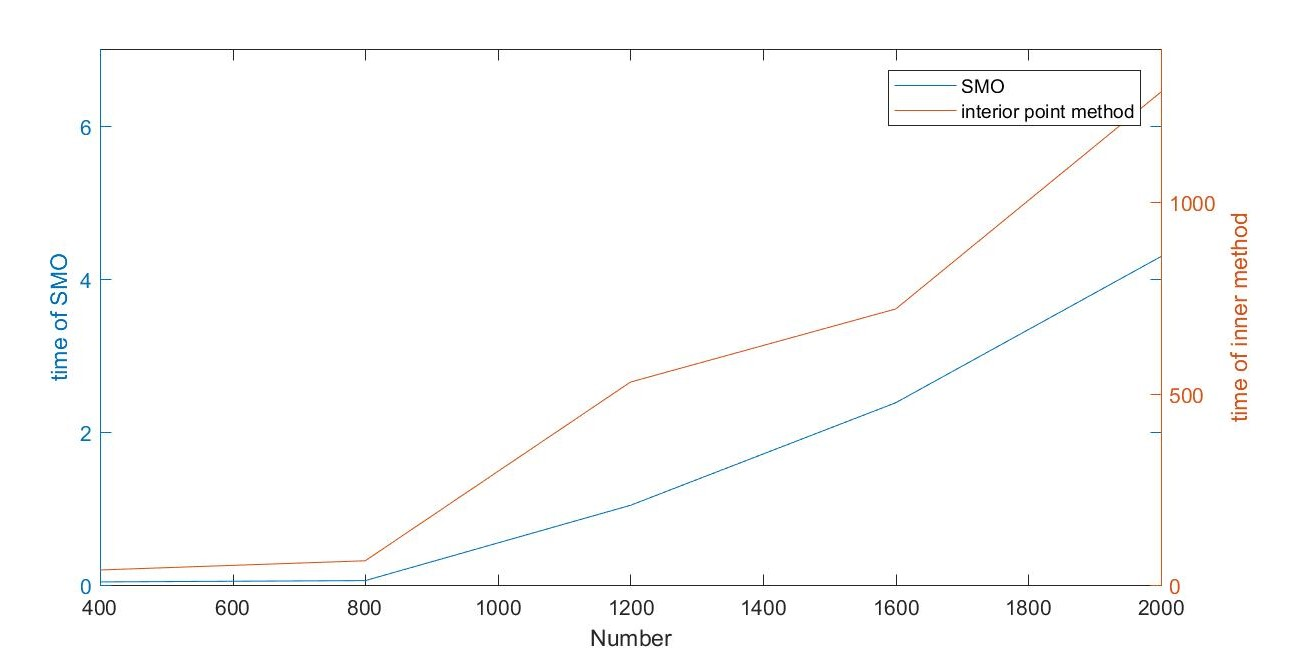
\includegraphics[height=7cm]{figure.jpg}
					\end{minipage}
				}
				\caption{Running time of two approaches}
			\end{figure}
	
	Running time of interior point method not only is hundred times bigger than that of SMO, but also increases quicker than SMO. In conclusion, for SVM, SMO is much useful than interior point method.

\end{document}